\section{Soft contrastive scores and Low-rank flow matching}

This note presents two approaches to estimating log likelihood ratios---and, from them, Hellinger distances--- contrastive method and flow matching with low-rank correction.

\subsection{Flow matching with low-dimensional correction term}

In the previous report, we presented flow matching with linear velocity $v = A(t)x + b(t,\theta)$. This method works fairly well; however, it still does not outperform the binning-and-classification (decoding) approach on periodic datasets. We suspect this is because the target distribution is not approximately Gaussian: the linear velocity approximation fails to capture non-Gaussian structure.

Therefore, we propose a velocity with a low-rank correction term (xflow\_sir\_lrank in figure \ref{fig:contrastive-soft-asset3}), $v = A(t)x + b(t,\theta) + U\,h_\phi(U^\top x, \theta, t)$, where $U \in \mathbb{R}^{d \times r}$ and $r \ll d$. $U$ can be a learnable matrix; alternatively, a more flexible approach is to let $U$ be learned by other means. From this perspective, $U$ identifies a subspace under a chosen objective, and the correction term learns the flow within that subspace.

When estimating the log likelihood ratio, we emphasize directions relevant to information coding---in particular, directions along which $\theta$ is more distinguishable. We therefore fit $U$ using the SIR method. In the simplest variant, SIR averages $x$ within each $\theta$ bin and then performs PCA on these averaged points; the columns of $U$ are the leading eigenvectors. $U$ is held fixed during training.

\subsection{Contrastive method}

Flow matching fits a velocity field and recovers log-density differences by integrating along the learned flow, so the likelihood ratio is only implicit in the training objective.

Contrastive method learns the log likelihood ratio more directly. The \texttt{contrastive\_soft} implementation learns a scalar score $S_\phi(x,\theta)=\exp(\rho)\,\langle g_{\phi_g}(x),\,h_{\phi_h}(\psi(\theta))\rangle$ from two MLP branches and a learned scale $\rho$, and minimizes an \emph{in-minibatch} cross-entropy between softmax probabilities $p_{ij}$ over batch candidates $\theta_j$ and soft targets $w_{ij}$.

Intuitively, for each $x_i$ the model should put predictive mass on batch stimuli $\theta_j$ close to the paired $\theta_i$, while farther batch entries act as implicit negatives.

After training, differences of $S_\phi(x,\cdot)$ across candidate stimuli estimate log-likelihood ratios (see \nameref{sss:contrastive-score-llr}).
\[
\log \frac{p(x\mid \theta_1)}{p(x\mid \theta_2)}
\approx
S_\phi(x,\theta_1)-S_\phi(x,\theta_2).
\]

\subsubsection{Results: Flow matching with low-rank correction performs well across datasets, espcially for two dimensional $\theta$ datasets}

We created four datasets: one-dimensional $\theta$ non-periodic, one-dimensional peridic, two-dimensional non-periodic, two-dimensional peridic. Each dataset contains five neurons, then projected to 30 dimensions using PR projection. This 30 dimensional embedding and $\theta$ values are datasets.

We applied flow matching with linear velocity and linear velocity with low-rank correction on these datasets. Both methods perform well in all datasets. And method with low-rank correction, however, does not perform particularly well compared with no low-rank correction.

Although, these flow matching methods still under perform binning and classification method on one-dimensional periodic datasets.

\subsubsection{Results: Using Fourier feature embedding improves flow matching method performance on periodic datasets.}

Instead of using raw $\theta$ as input, we use Fourier features of $\theta$ as input. This method performs well on one-dimensional periodic datasets.

\subsubsection{Results: Contrastive method performs well on non-periodic datasets}

\subsubsection{Results: Contrastive method performs well on one-dimensional periodic datasets only when using Fourier feature embedding}

However, still underperform binning and classification method on periodic datasets.

\begin{figure}[!htbp]
  \centering
  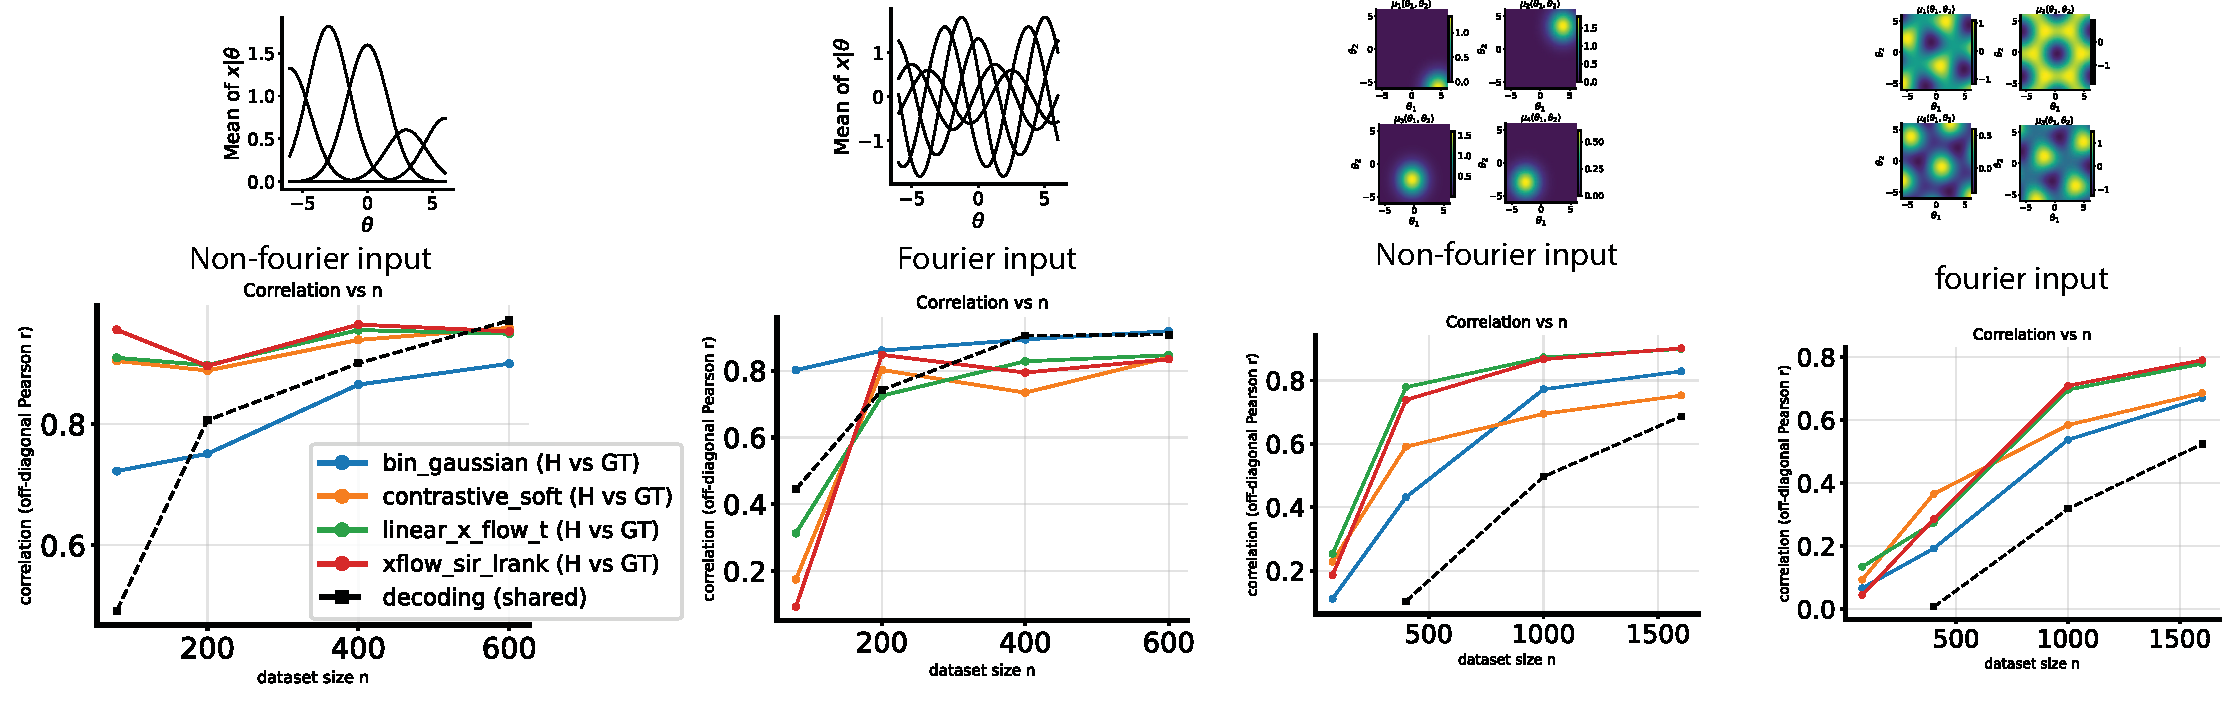
\includegraphics[width=\linewidth]{notes/figures/2026-05-06-contrastive/asset3.pdf}
  \caption{%
  Comparison of several methods across datasets. \emph{bin\_gaussian:} bin the data, estimate bin means $\mu$, pool residuals $x-\mu$ across bins to fit a single diagonal covariance, form a Gaussian model, and evaluate the Hellinger distance in closed form. \emph{contrastive\_soft:} score $g(x)^\top h(\theta)$ with neural $g,h$; maximize scores on soft positive pairs (kernel-defined). \emph{linear\_x\_flow\_t:} flow matching with velocity $v = A(t)x + b(t,\theta)$. \emph{xflow\_sir\_lrank:} $v = A(t)x + b(t,\theta) + U\,h(U^\top x)$, where columns of $U$ are raw SIR directions fit on the training split. \emph{Fourier input} maps $\theta$ to Fourier features (four frequency pairs) plus a linear term, producing $\tilde{\theta}$ input for the network; \emph{non-Fourier input} passes $\theta$ directly. Top row: example neuron tuning curves per dataset. Observations live in five intrinsic dimensions (five neurons) embedded into $30$ via PR projection.
  }
  \label{fig:contrastive-soft-asset3}
\end{figure}

\pagebreak

\subsection{Methods}

\subsubsection{Likelihood-ratio interpretation}\label{sss:contrastive-score-llr}

For hard in-batch contrastive learning, a Bayes-optimal score against proposals drawn from $q(\theta)$ can be written as
\[
S^*(x,\theta)=\log \frac{p(\theta\mid x)}{q(\theta)}+C(x),
\]
where $q(\theta)$ is the negative-sampling distribution and $C(x)$ does not depend on $\theta$.
By Bayes' rule,
\[
S^*(x,\theta)
=
\log p(x\mid \theta)
+
\log p_{\mathrm{train}}(\theta)
-
\log q(\theta)
+
C'(x),
\]
where $p_{\mathrm{train}}$ denotes the marginal distribution of $\theta$ in the training data (empirically, the distribution from which batch stimuli are drawn).

Fixing $x$ and comparing two candidates $\theta_1,\theta_2$ eliminates the $x$-dependent constants:
\[
\log \frac{p(x\mid \theta_1)}{p(x\mid \theta_2)}
=
S^*(x,\theta_1)-S^*(x,\theta_2)
-
\log \frac{p_{\mathrm{train}}(\theta_1)}{p_{\mathrm{train}}(\theta_2)}
+
\log \frac{q(\theta_1)}{q(\theta_2)}.
\]
In our in-minibatch setup, negative $\theta$ values are other stimuli appearing in the same batch, so at the level of the training distribution $q(\theta)=p_{\mathrm{train}}(\theta)$ and the last two terms cancel. Replacing $S^*$ by the learned $S_\phi$ yields the approximation
\[
\log \frac{p(x\mid \theta_1)}{p(x\mid \theta_2)}
\approx
S_\phi(x,\theta_1)-S_\phi(x,\theta_2).
\]

\subsubsection{Divergence for \texttt{xflow\_sir\_lrank}}

The scheduled velocity field has the form
\[
v(x,t,\theta)=A(t)x+b(t,\theta)+U\,h_\phi\!\bigl(U^{\mathsf T}x,\,t,\,\theta\bigr),
\qquad z:=U^{\mathsf T}x\in\mathbb{R}^{r},
\]
with fixed raw SIR directions stored as the columns of $U\in\mathbb{R}^{d\times r}$ (held constant during training).
For linear $x$-flow with symmetric $A(t)$, the divergence splits into a linear part and the correction:
\[
\nabla_x\!\cdot v
=
\mathrm{tr}\,A(t)
+
\nabla_x\!\cdot\bigl(U\,h_\phi(z,t,\theta)\bigr).
\]
Because $U$ does not depend on $x$, the Jacobian of the correction is $U\,(\partial h_\phi/\partial z)\,U^{\mathsf T}$, hence
\[
\nabla_x\!\cdot\bigl(U\,h_\phi\bigr)
=
\mathrm{tr}\!\left(U^{\mathsf T}U\,\frac{\partial h_\phi}{\partial z}\right).
\]
If $U$ has orthonormal columns, $U^{\mathsf T}U=I_r$ and the correction contribution reduces to $\mathrm{tr}\,(\partial h_\phi/\partial z)$.
For raw SIR components, $U$ need not be orthogonal; we therefore use the Gram matrix $G:=U^{\mathsf T}U\in\mathbb{R}^{r\times r}$ and evaluate $\mathrm{tr}(G\,\partial h_\phi/\partial z)$.

In the implementation, $h_\phi$ is an MLP on $(z,t,\theta)$ and autograd is applied only through $z$.
Concretely, $z$ is formed from $x$ and then treated as an independent variable with $\partial h_\phi/\partial z$ computed by reverse-mode differentiation.

The trace $\mathrm{tr}(G\,\partial h_\phi/\partial z)$ is estimated in one of two ways.
\emph{Exact} mode loops over output indices $j=1,\ldots,r$, forming $\partial h_{\phi,j}/\partial z\in\mathbb{R}^{r}$ for each $j$ and accumulating $\sum_{k=1}^{r} G_{jk}\,(\partial h_{\phi,j}/\partial z_k)$, which equals $\mathrm{tr}(G\,\partial h_\phi/\partial z)$ when $G$ is symmetric.
\emph{Hutchinson estimator}.

\subsubsection{\texttt{contrastive\_soft}}

During preprocessing, we whiten the data using the training split only: each coordinate of $x$ and of $\theta$ is centered and divided by its empirical standard deviation (with a floor on the $\theta$ scales). The resulting location and scale pairs $(\mu_x,\sigma_x)$ and $(\mu_\theta,\sigma_\theta)$ are then fixed and reused at validation time and when forming decoding matrices.

The preprocessed inputs are then passed through two MLPs, $g_{\phi_g}$ and $h_{\phi_h}$, to produce a scalar score 
\[
S_\phi(x,\theta)=\alpha\,\big\langle g_{\phi_g}(x),\,h_{\phi_h}(\theta)\big\rangle,\qquad \alpha=\exp(\rho),
\]
with a scalar $\rho$ learned jointly with the networks.

Each training step uses a minibatch of $B\ge 2$ paired draws: observations $x_1,\ldots,x_B$ with matching stimuli $\theta_1,\ldots,\theta_B$. For each index $i$, we define the predicted probabilities $p_{ij}=\mathrm{softmax}_j(S_\phi(x_i,\theta_j))$.

We define soft target probabilities
\[
w_{ij}=\frac{\exp\big(-d_{ij}^2/(2h^2)\big)}{\sum_{k=1}^B \exp\big(-d_{ik}^2/(2h^2)\big)},
\]
where $d_{ij}=\mathrm{dist}(\theta_i,\theta_j)$ is the Euclidean distance between $\theta_i$ and $\theta_j$.
We set $h$ to the $\theta$-range divided by twice the number of bins.

Finally, parameters are updated by minimizing the loss
\[
\mathcal{L}(\phi)=-\frac{1}{B}\sum_{i=1}^B\sum_{j=1}^B w_{ij}\,\log p_{ij}.
\]
If $h$ is small compared with typical within-batch separations, then, for each $i$, the weights $w_{ij}$ concentrate on $j=i$ and the objective collapses to the usual hard InfoNCE / multiclass contrastive loss with a one-hot target on the diagonal.

\subsubsection{Two-dimensional non-periodic (random-amplitude Gaussian bumps).}
The two-coordinate analogue of the scalar Gaussian-bump family replaces the stimulus by $\theta=(\theta_1,\theta_2)^{\mathsf{T}}$ on a bounded rectangle (no wrapping).
Joint stimuli are drawn independently from a uniform density on $[\theta_{\mathrm{low}},\theta_{\mathrm{high}}]^2$, matching the interval endpoints used in the one-dimensional recipe.

Before drawing joint samples $(\theta,x)$, we sample one amplitude per coordinate,
\begin{equation}
  a_j \sim \mathrm{Uniform}(a_{\mathrm{low}}, a_{\mathrm{high}}),
  \qquad j = 1,\ldots,d,
\end{equation}
independently across $j$, and one planar tuning center per coordinate,
\begin{equation}
  c_j \sim \mathrm{Uniform}\bigl([\theta_{\mathrm{low}},\theta_{\mathrm{high}}]^2\bigr),
  \qquad j = 1,\ldots,d,
\end{equation}
independently across $j$.
The vectors $(a_1,\ldots,a_d)$ and $(c_1,\ldots,c_d)$ are held fixed across the dataset.

Given $\theta$, the conditional mean of $x_j$ is an isotropic Gaussian bump in the stimulus plane centered at $c_j$,
\begin{equation}
  \mu_j(\theta)
  =
  a_j \exp\!\bigl(-\kappa\,\|\theta-c_j\|^2\bigr),
  \qquad j = 1,\ldots,d,
\end{equation}
with bump precision $\kappa\ge 0$, and $\mu(\theta)=(\mu_1(\theta),\ldots,\mu_d(\theta))^{\mathsf{T}}$.
Conditionally on $\theta$, the observation is multivariate Gaussian with diagonal covariance using the same additive $\sqrt{d}$ variance law as in the scalar non-periodic generator (baseline scales per coordinate, activity weights, and optional jitter), so $|\mu_j(\theta)|$ enters additively in the per-coordinate variance alongside the scaled baseline term.

\subsubsection{Two-dimensional periodic (three-orientation grid cosine tuning).}
The two-coordinate periodic analogue replaces Gaussian bumps by random-gain cosine tuning built from three wavevectors in the $(\theta_1,\theta_2)$ plane, analogous to how the scalar periodic family replaces bumps by cosines along a single stimulus axis.
As in the one-dimensional cosine experiment, stimuli are drawn uniformly on a bounded square; the conditional means are periodic functions of $\theta$ even though $\theta$ itself is not wrapped.

Before drawing joint samples $(\theta,x)$, sample one gain per coordinate,
\begin{equation}
  a_j \sim \mathrm{Uniform}(a_{\mathrm{low}}, a_{\mathrm{high}}),
  \qquad j = 1,\ldots,d,
\end{equation}
independently across $j$, one orientation offset per coordinate,
\begin{equation}
  \rho_j \sim \mathrm{Uniform}(0,\pi/3),
  \qquad j = 1,\ldots,d,
\end{equation}
and three phases per coordinate,
\begin{equation}
  \phi_{j,m}\sim \mathrm{Uniform}(0,2\pi),
  \qquad m\in\{1,2,3\},
\end{equation}
with fixed angular spacing $\pi/3$ defining three wavevectors $k_{j,m}$ from $\rho_j$ and a stimulus-axis frequency $\omega_j>0$ (typically $\omega_j=1$ in the bundled recipes).
The vector of gains $(a_1,\ldots,a_d)$ and the orientation and phase arrays are held fixed across samples.

Given $\theta$, the conditional mean averages three cosines,
\begin{equation}
  \mu_j(\theta)
  =
  \frac{a_j}{3}\sum_{m=1}^{3}\cos\!\bigl(k_{j,m}^{\mathsf{T}}\theta+\phi_{j,m}\bigr),
  \qquad j = 1,\ldots,d,
\end{equation}
and $\mu(\theta)=(\mu_1(\theta),\ldots,\mu_d(\theta))^{\mathsf{T}}$.
The observation noise uses the same diagonal Gaussian construction as in the non-periodic two-coordinate family.


\subsection{Supplementary}

\subsubsection{}

\begin{figure}[!htbp]
  \centering
  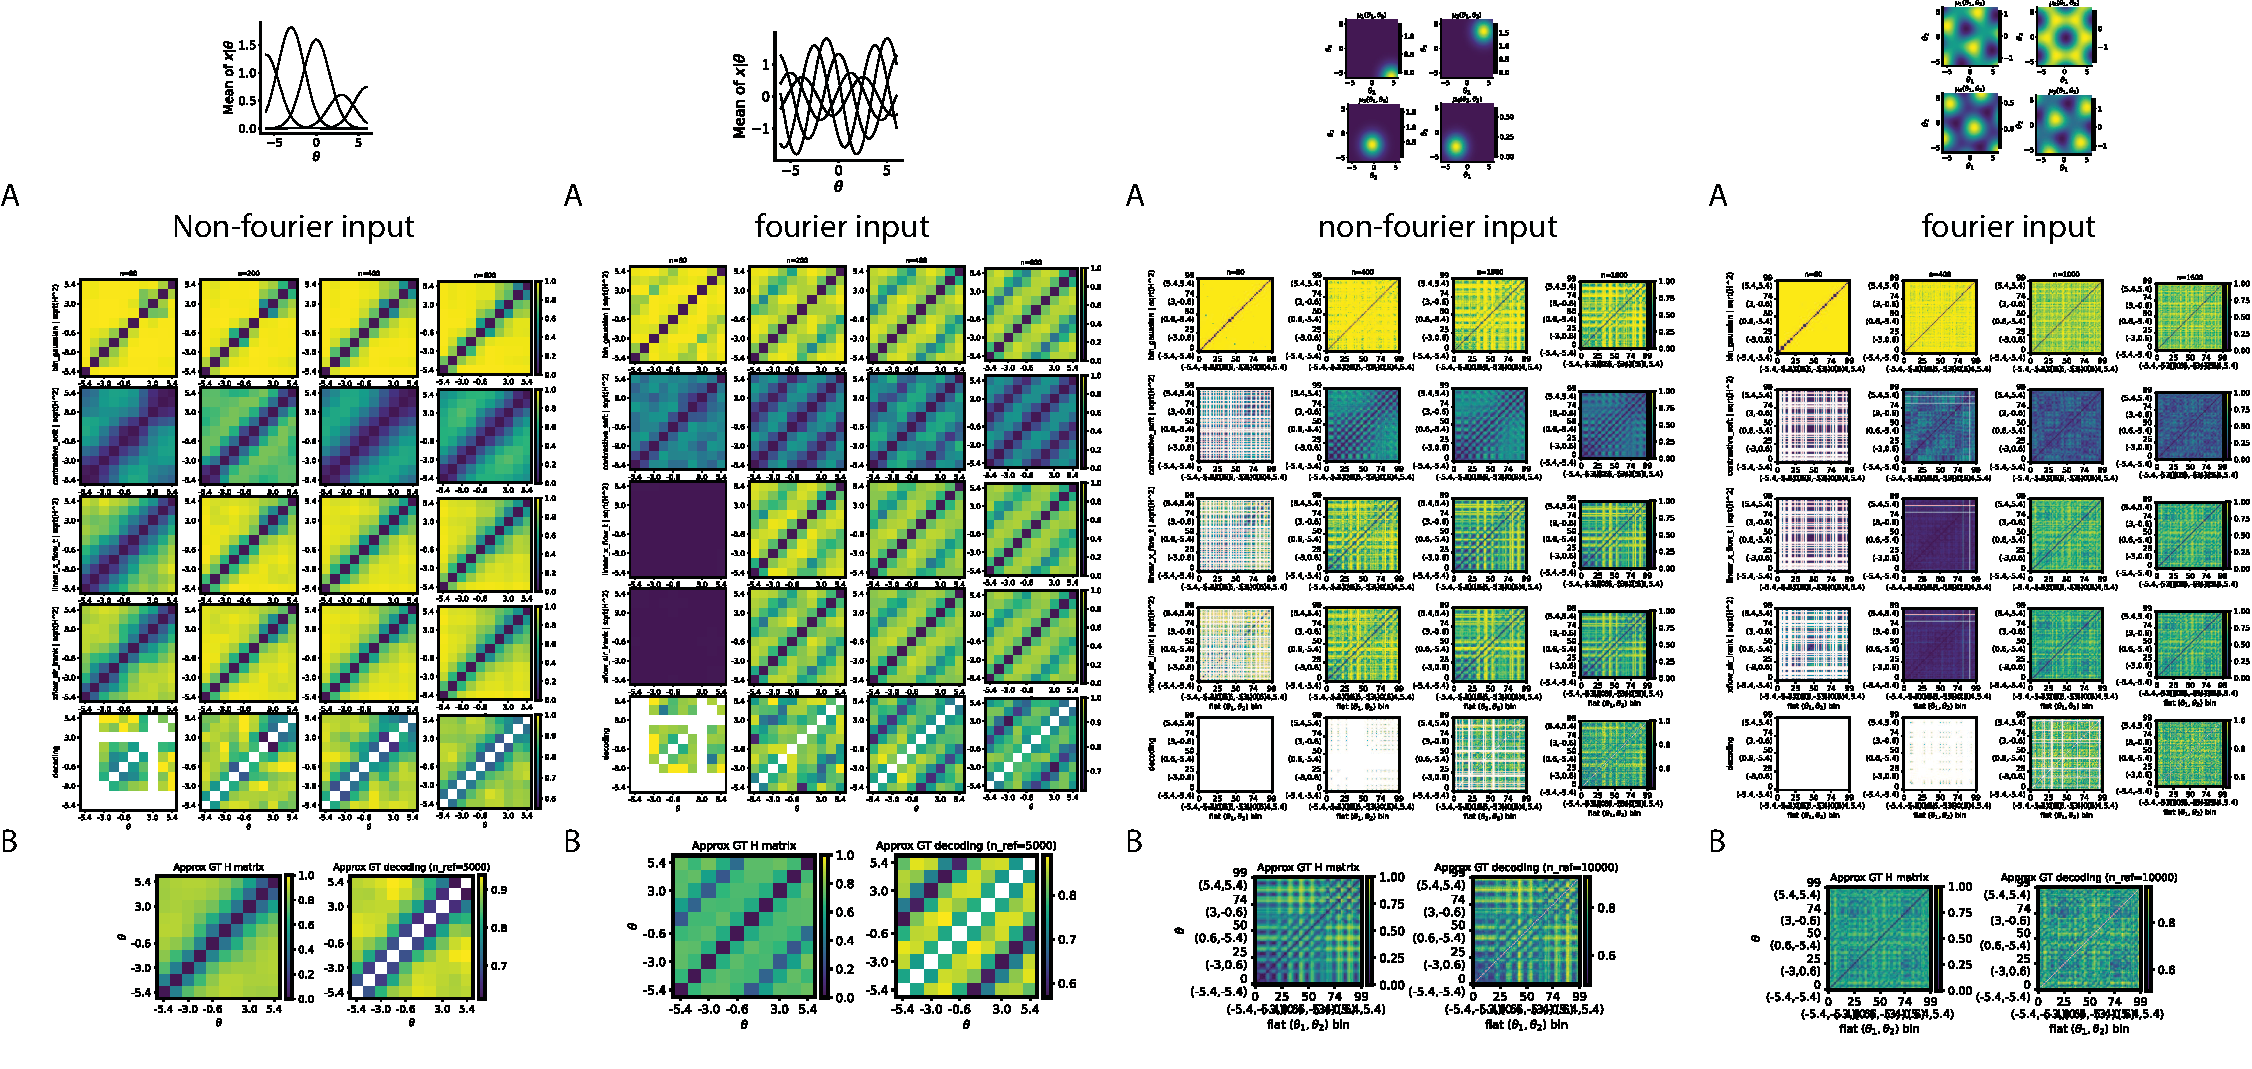
\includegraphics[width=\linewidth]{notes/figures/2026-05-06-contrastive/asset2.pdf}
  \caption{%
  Composite panels for soft contrastive decoding and related baselines (axis labels and panel letters are in the figure).
  }
  \label{fig:contrastive-soft-asset2}
\end{figure}

\FloatBarrier

\FloatBarrier
\begin{figure}[!htbp]
  \centering
  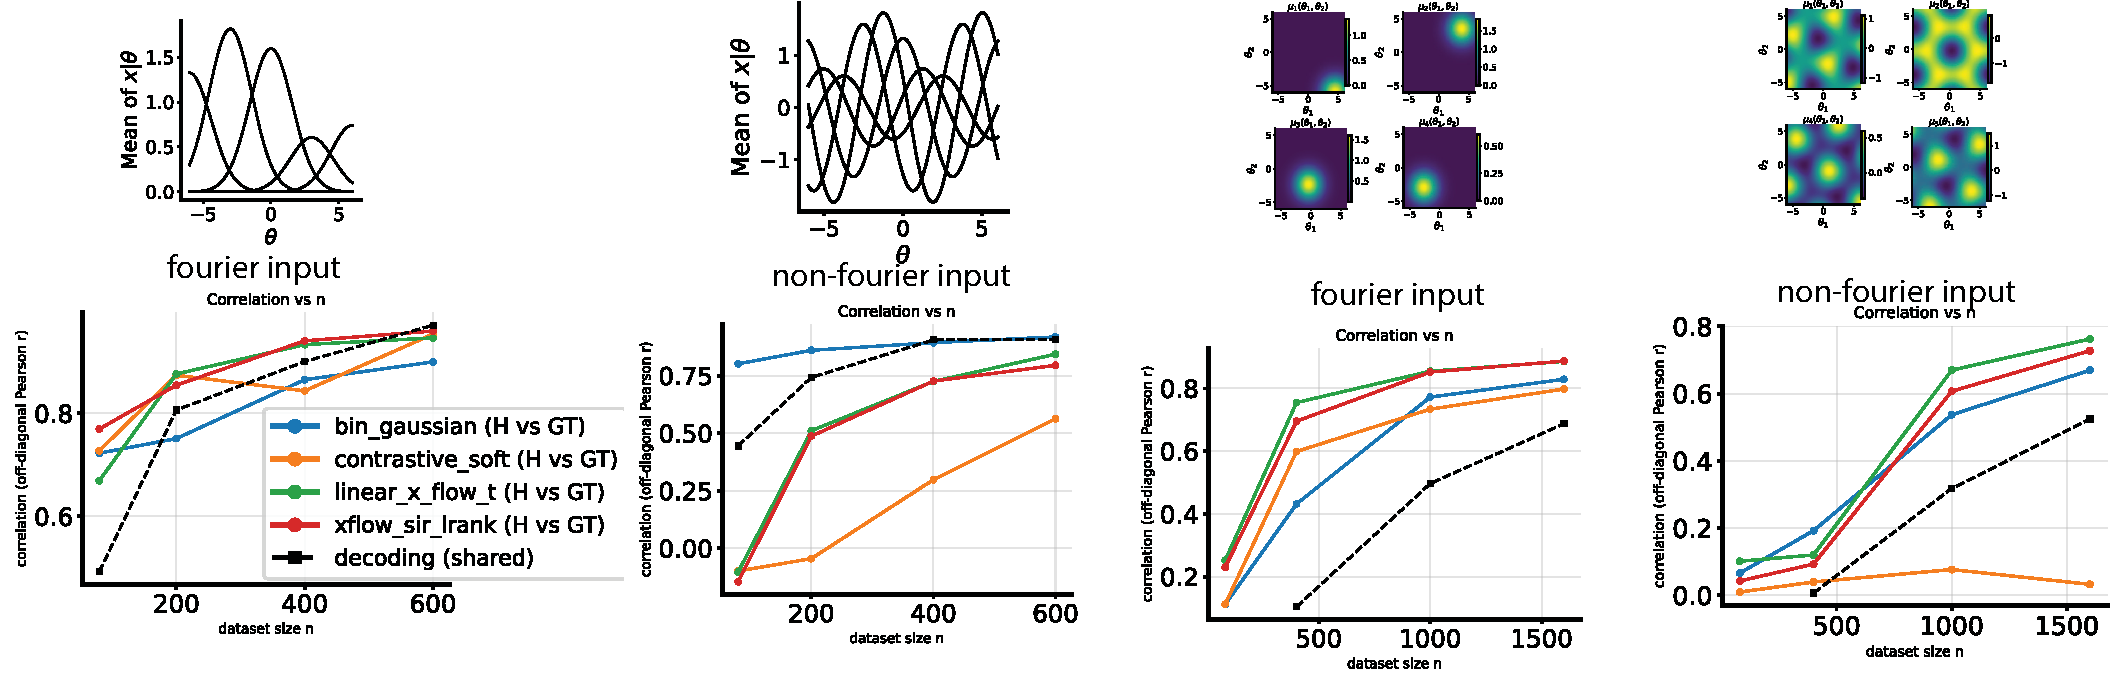
\includegraphics[width=\linewidth]{notes/figures/2026-05-06-contrastive/asset4.pdf}
  \caption{%
  Additional diagnostics in the same study (see in-figure annotations).
  }
  \label{fig:contrastive-soft-asset4}
\end{figure}

\FloatBarrier
\begin{figure}[!htbp]
  \centering
  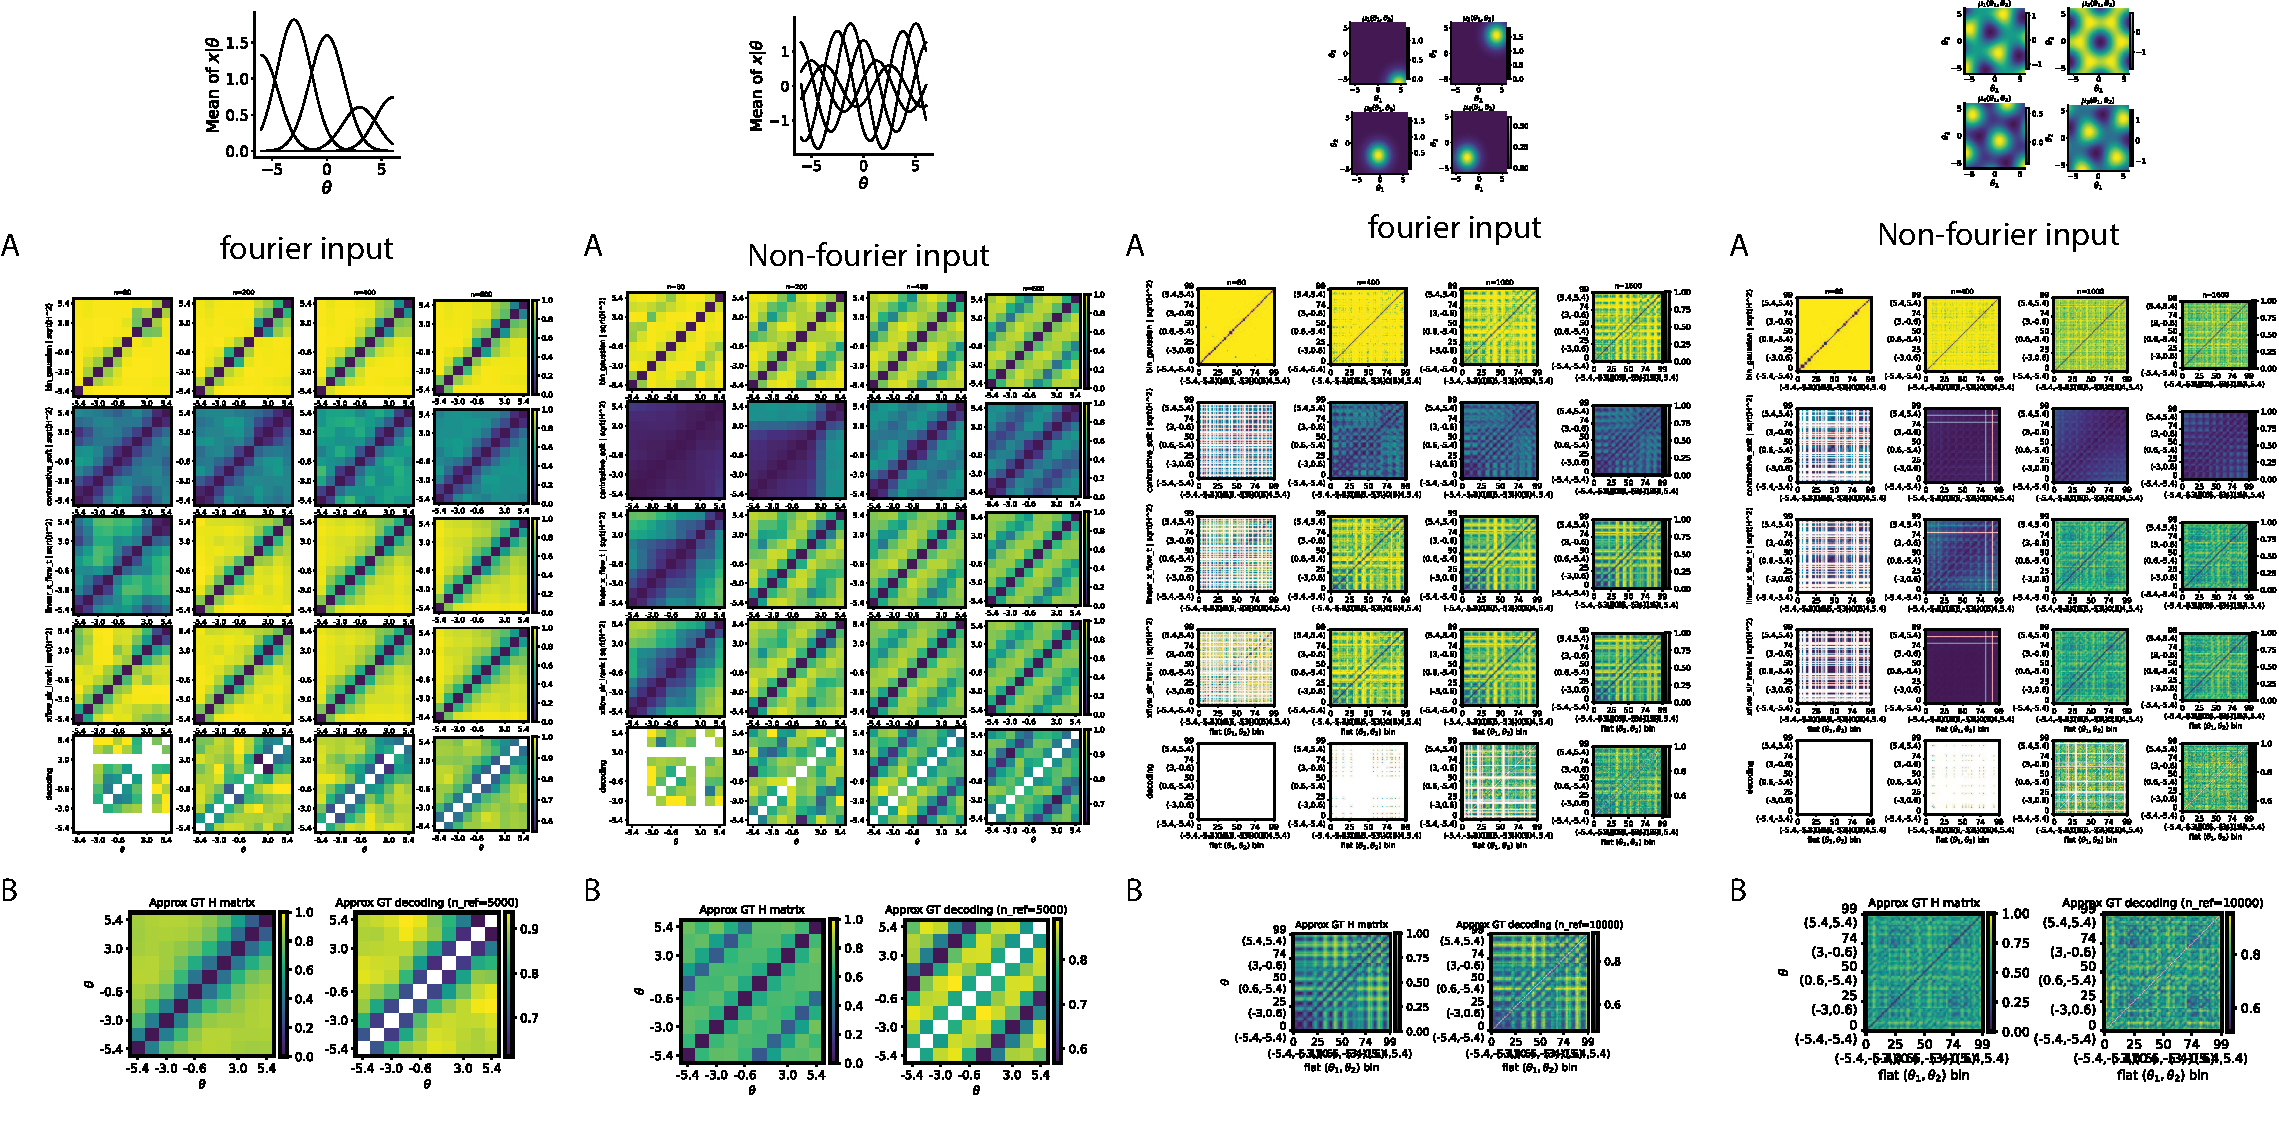
\includegraphics[width=\linewidth]{notes/figures/2026-05-06-contrastive/asset5.pdf}
  \caption{%
  Additional composite summary (see in-figure annotations).
  }
  \label{fig:contrastive-soft-asset5}
\end{figure}

\FloatBarrier
